%%% Template originaly created by Karol Kozioł (mail@karol-koziol.net) and modified for ShareLaTeX use

\documentclass[a4paper,11pt]{article}

\usepackage[T1]{fontenc}
\usepackage[utf8]{inputenc}
\usepackage{graphicx}
\usepackage{xcolor}

%\renewcommand\familydefault{\sfdefault}
\usepackage{lmodern}
\usepackage{booktabs}
\usepackage{amsmath,amssymb,amsthm,textcomp}
\usepackage{enumerate}
\usepackage{multicol}
\usepackage{tikz}

\usepackage{geometry}
\geometry{left=25mm,right=25mm,%
bindingoffset=0mm, top=20mm,bottom=20mm}


\linespread{1.3}

\newcommand{\linia}{\rule{\linewidth}{0.5pt}}

% custom theorems if needed
\newtheoremstyle{mytheor}
    {1ex}{1ex}{\normalfont}{0pt}{\scshape}{.}{1ex}
    {{\thmname{#1 }}{\thmnumber{#2}}{\thmnote{ (#3)}}}

\theoremstyle{mytheor}
\newtheorem{defi}{Definition}

% my own titles
\makeatletter
\renewcommand{\maketitle}{
\begin{center}
\vspace{2ex}
{\huge \textsc{\@title}}
\vspace{1ex}
\\
\linia\\
\@author \hfill \@date
\vspace{1ex}
\end{center}
}
\makeatother
%%%

% custom footers and headers
\usepackage{fancyhdr}
\pagestyle{fancy}
\lhead{}
\chead{}
\rhead{}
\lfoot{CID: 01343907}
\cfoot{Time Series Analysis Coursework}
\rfoot{Page \thepage}
\renewcommand{\headrulewidth}{0pt}
\renewcommand{\footrulewidth}{0.5pt}
%

% code listing settings
\usepackage{listings}
\lstset{
    language=Python,
    basicstyle=\ttfamily\small,
    aboveskip={1.0\baselineskip},
    belowskip={1.0\baselineskip},
    columns=fixed,
    extendedchars=true,
    breaklines=true,
    tabsize=4,
    prebreak=\raisebox{0ex}[0ex][0ex]{\ensuremath{\hookleftarrow}},
    frame=lines,
    showtabs=false,
    showspaces=false,
    showstringspaces=false,
    keywordstyle=\color[rgb]{0.627,0.126,0.941},
    commentstyle=\color[rgb]{0.133,0.545,0.133},
    stringstyle=\color[rgb]{01,0,0},
    numbers=left,
    numberstyle=\small,
    stepnumber=1,
    numbersep=10pt,
    captionpos=t,
    escapeinside={\%*}{*)}
}

%%%----------%%%----------%%%----------%%%----------%%%

\begin{document}

\title{Time Series Analysis Coursework 2020-2021}

\author{Juliette Limozin, CID: 01343907}

\date{Due 18/12/2020 at 4 pm}

\maketitle

\section*{Question 1}
\subsection*{(a)}

\begin{lstlisting}
def S_AR(f,phis,sigma2):
    """
    INPUTS
    f: a vector of frequencies at which to evaluate the spectral density function.
    phis: the vector [φ1,p, ..., φp,p].
    sigma2: the variance of the white noise.
    OUTPUT:
    S: a vector of values of the spectral density function evaluated at the elements of f.
    """
    if str(type(phis)) != "<class 'numpy.ndarray'>" :
        raise ValueError('Please input a numpy array for phis')
    p = len(phis) #Determine p
    A = np.concatenate((np.array([1]), -phis), axis = 0)
    exps = np.exp(-1j*2*np.pi*np.asarray(range(0,p+1), dtype = 'complex'))
    S = [sigma2/np.dot(A, exps**i) for i in f]
    
    return S
\end{lstlisting}

\subsection*{(b)}

\begin{lstlisting}
def AR2_sim(phis,sigma2,N):
    et = np.random.normal(0, np.sqrt(sigma2), 100+N)
    X = np.zeros(100+N)
    for t in range(2,100+N):
        X[t] = phis[0]*X[t-1]+phis[1]*X[t-2]+et[t]
    
    X = X[100:]
    
    return X
\end{lstlisting}

\subsection*{(c)}
\begin{lstlisting}
def acvs_hat(X,tau):
    N = len(X)
    s = np.zeros(len(tau))
    for i in range(len(tau)):
        s[i] = (1/N)*np.dot(X[:N-tau[i]], X[tau[i]:])
    
    return s
\end{lstlisting}
\newpage

\section*{Question 2}

\subsection{(a)}

\begin{lstlisting}
def periodogram(X):
    N = len(X)
    S = (1/N)*np.abs(fft(X))**2
    
    return S

def direct(X):
    N = len(X)
    t = np.array(range(1,N+1))
    h = 0.5*(8/(3*(N+1)))**0.5 * (1-np.cos(2*np.pi*t/(N+1)))
    
    S = (1/N)*np.abs(fft(np.multiply(h,X)))**2
    
    return S
\end{lstlisting}


\newpage

\section*{Question 3}
\subsection*{(a)}

Figure \ref{plot3a} shows the plots of the periodogram and the direct spectral estimate using the Hanning taper of my time series.

\begin{figure}[h!]
    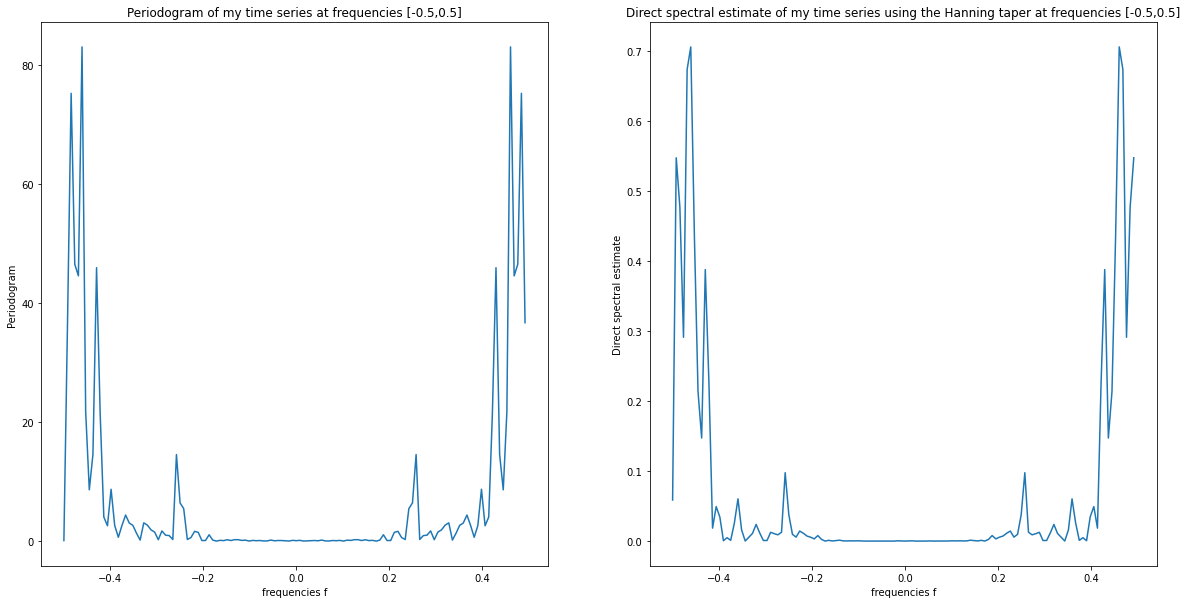
\includegraphics[width=\columnwidth]{plot3a.png}
    \caption{Plots for Question 3(a)}
    \label{plot3a}
\end{figure}

\subsection*{(b)}

The following is my code for fitting a AR(p) model using the Yule-Walker, Least Squares and approximate maximum likelihood methoods. 

\begin{lstlisting}
def yule_walker(X,p):
    s_hat = acvs_hat(X, list(range(0,p+1)))
    gamma = s_hat[1:]
    Gamma = toeplitz(s_hat[:-1], s_hat[:-1])
    phi_hat = np.linalg.inv(Gamma).dot(gamma)
    sigma2_hat = s_hat[0] - np.dot(phi_hat,s_hat[1:])
    
    return phi_hat, sigma2_hat

def least_squares(X,p):
    N = len(X)
    F = np.zeros((N-p,p))
    for i in range(p):
        F[:,i] = X[(p-i-1):(N-1-i)]
    phi_hat = np.linalg.inv(F.T.dot(F)).dot(F.T).dot(X[p:])
    sigma2_hat = (1/(N-2*p))*(X[p:]-F.dot(phi_hat)).T.dot(X[p:]-F.dot(phi_hat))
    
    return phi_hat, sigma2_hat

def approx_mle(X,p):
    N = len(X)
    phi_hat, sigma2_hat = least_squares(X, p)
    sigma2_hat = sigma2_hat *(N-2*p)/(N-p)
    
    return phi_hat, sigma2_hat
\end{lstlisting}

\subsection*{(c)}

The information on the AIC for each model method and parameter is summarised in the table below. \\

\begin{tabular}{lrrr}
\toprule
{} &  Yule-Walker &  Least Squares &  Approximate MLE \\
\midrule
p = 1  &    83.457568 &      79.308525 &        78.296662 \\
p = 2  &    67.210892 &      62.744916 &        60.696873 \\
p = 3  &    42.897565 &      35.014882 &        31.905417 \\
p = 4  &    10.712505 &     -22.692807 &       -26.889905 \\
p = 5  &    11.667585 &     -23.526619 &       -28.838585 \\
p = 6  &    12.558746 &     -19.564828 &       -26.019978 \\
p = 7  &    13.945686 &     -16.908833 &       -24.536622 \\
p = 8  &    15.673155 &     -13.065779 &       -21.896866 \\
p = 9  &    16.615987 &     -11.939696 &       -22.006017 \\
p = 10 &    18.121540 &     -11.858851 &       -23.193686 \\
p = 11 &    19.796076 &      -7.995110 &       -20.633170 \\
p = 12 &    21.759412 &      -7.187960 &       -21.165469 \\
p = 13 &    22.142904 &      -5.101213 &       -20.456005 \\
p = 14 &    23.842761 &      -3.255814 &       -20.027431 \\
p = 15 &    25.429476 &       0.521702 &       -17.708102 \\
p = 16 &    26.306425 &       2.717655 &       -17.013632 \\
p = 17 &    26.731132 &       3.343002 &       -17.935132 \\
p = 18 &    28.727868 &       5.515377 &       -17.357172 \\
p = 19 &    30.279313 &       8.161516 &       -16.355375 \\
p = 20 &    31.917098 &      12.468884 &       -13.744801 \\
\bottomrule
\end{tabular}

\subsection*{(d)}
We choose the order of model with the lowest AIC score for each method.

Hence we choose $p = 4$ for the Yule-Walker model, and $p=5$ for both the Least Squares and approximate maximum likelihood models.

The corresponding parameter estimates are shown in the table below, up to 4 decimal points. \\

\begin{tabular}{llll}
\toprule
{} &Yule-Walker & Least Squares & Approximate MLE \\
\midrule
$\hat{\mathbf{\phi}}$    &  \parbox{3cm}{[-1.5452, -1.2955, -1.0781, -0.4841]} &  \parbox{3.75cm}{[-1.7241, -1.6180, -1.4260, -0.7367, -0.0647]} &  \parbox{3.75cm}{[-1.7241, -1.6180, -1.4260, -0.7367, -0.0647]} \\
$\hat{\sigma}^2$ &  1.0214 &  0.7696 &  0.7383 \\
\bottomrule
\end{tabular}

\subsection*{(e)}

Figure \ref{plot3e} shows the associated spectral density function for each of the three selected models.

\begin{figure}[h!]
    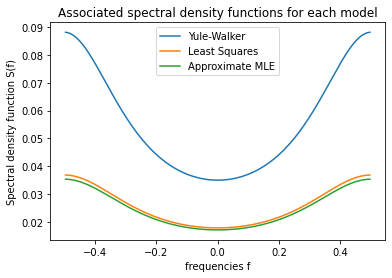
\includegraphics{plot_3e.png}
    \caption{Plot for Question 3(e)}
    \label{plot3e}
\end{figure}
\end{document}
